\section{Introduction}

FLEX conducts the lexical analysis of the input stream.
\begin{definition}[\textit{Lexical analysis}]
    Lexical analysis pertains to the vocabulary or words of a language, distinct from its grammar and structure.
\end{definition}

In natural languages, words can be straightforwardly listed, but this enumeration isn't feasible for artificial languages. 
For instance, in the C programming language, identifiers must adhere to the following rules:
\begin{itemize}
    \item They consist of a sequence of alphanumeric characters (including underscore $\_$).
    \item They cannot commence with a digit.
\end{itemize}
Technical terms are less intricate than natural language words: their structure is simpler, they adhere to specific rules, and they typically conform to a regular language.

\subsection{Lexical analysis}
A lexical analysis is responsible for identifying tokens within a sequence of characters, such as identifiers and constants. 
It may also augment tokens with supplementary information like identifier names and line-by-line positions. 
Typically, this analysis is conducted using a scanner, although manually coding a scanner can be laborious and prone to errors. 
Thankfully, there are scanner generators like FLEX, which operate on regular expression descriptions to automate this process. 
Essentially, a scanner can be conceptualized as a comprehensive finite state automaton.

In certain scenarios, a scanner suffices as it can identify words and execute semantic actions like local transformations. 
However, in the context of a compiler, the scanner serves a broader purpose. 
It primes the input for the parser by identifying language tokens such as identifiers, constants, keywords, and punctuation. 
Additionally, it cleanses the input by removing comments and enriches tokens with essential information like lexical values and locations.

The workflow of FLEX is shown in the following image. 
\begin{figure}[H]
    \centering
    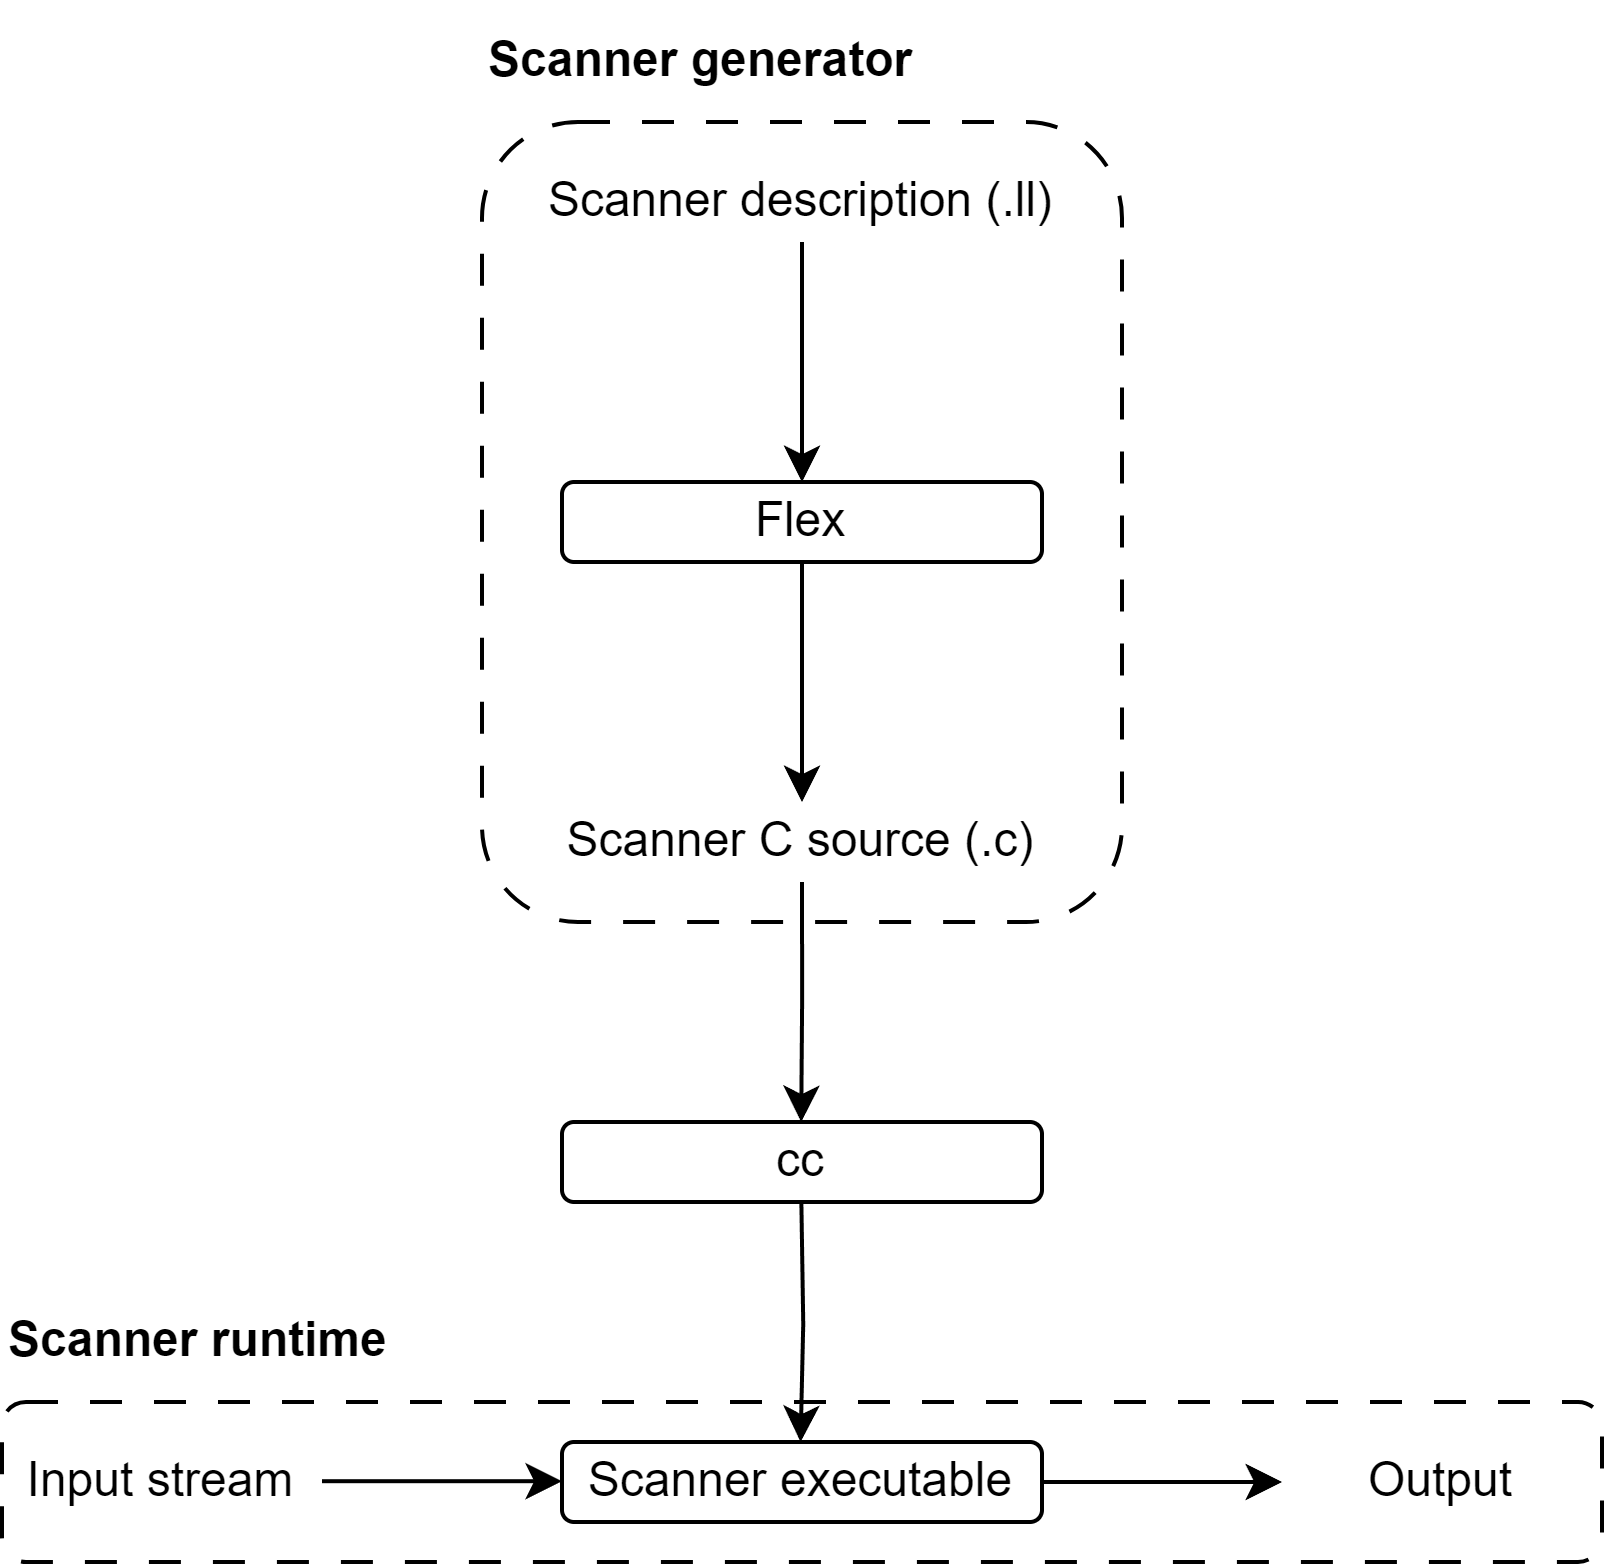
\includegraphics[width=0.39\linewidth]{images/flex.png}
    \caption{FLEX workflow}
\end{figure}